\chapter{appendix}\label{chapter:appendixA}


\section{Hidden Markov Model\cite{jurafsky2000speech}}


The \textbf{Hidden Markov Model(HMM)} is based on augmenting the Markov chain. A \textbf{Markov chain} is a model that tells us something about the probabilities of sequences of random variables,
states, each of which can take on values from some set. These sets can be words, or
tags, or symbols representing anything, like the weather. A Markov chain makes a
very strong assumption that if we want to predict the future in the sequence, all that
matters is the current state. The states before the current state have no impact on the
future except via the current state. More formally, consider a sequence of state variables $q_1,q_2,\dots,q_i$. A Markov model embodies the Markov assumption on the probabilities of this sequence: that Markov assumption when predicting the future, the past doesn’t matter, only the present.

$$\text{Markov assumption:} P(q_i= a|q_1,q_2,\dots,q_{i-1}) = P(q_i=a|q_{i-1})$$

A Markov chain is useful when we need to compute a probability for a sequence of observable events. In many cases, however, the events we are interested in are hidden: we don't observe them directly. For example, we don't normally observe part-of-speech tags in a text. Rather, we see words, and must infer the tags from the word sequence. We call the tags hidden because they are not observed. 

A hidden Markov model (HMM) allows us to talk about both \textit{observed} events (like words that we see in the input) and \textit{hidden} events (like part-of-speech tags) that we think of as causal factors in our probabilistic model. An HMM is specified by the following components:



\clearpage
\begin{table}[h!]
\centering
\renewcommand{\arraystretch}{1.5}
\begin{tabular}{>{\centering\arraybackslash}m{3cm}  >{\arraybackslash}m{9cm} }
\toprule
\textbf{Symbol} & \textbf{Description} \\ 
\midrule
$Q = q_1 q_2 \cdots q_N$ & A set of $N$ states \\ 
\midrule
$A = a_{11} \cdots a_{ij} \cdots a_{NN}$ & A \textbf{transition probability matrix} $A$, where each $a_{ij}$ represents the probability of moving from state $i$ to state $j$, such that $\sum_{j=1}^{N} a_{ij} = 1, \, \forall i$ \\ 
\midrule
$B = b_i(o_t)$ & A sequence of \textbf{observation likelihoods}, also called \textbf{emission probabilities}, each expressing the probability of an observation $o_t$ (drawn from a vocabulary $V = \{v_1, v_2, \ldots, v_V\}$) being generated from a state $q_i$ \\ 
\midrule
$\pi = \pi_1, \pi_2, \ldots, \pi_N$ & An \textbf{initial probability distribution} over states. $\pi_i$ is the probability that the Markov chain will start in state $i$. Some states $j$ may have $\pi_j = 0$, meaning that they cannot be initial states. Also, $\sum_{i=1}^{n} \pi_i = 1$ \\ 
\bottomrule
\end{tabular}
\caption{Hidden Markov Model Parameters}
\end{table}


The HMM is given as input $O=o_1o_2 \dots o_T$: a sequence of $T$ observations, each
one drawn from the vocabulary $V$.
A first-order hidden Markov model instantiates two simplifying assumptions.
\begin{itemize}
    \item First, as with a first-order Markov chain, the probability of a particular state depends only on the previous state.
    \item Second, the probability of an observation depends only on the state that produced the observation. The model is defined by the following parameters.
\end{itemize}




\chapter{Figures}\label{chapter:appendixB}

\section{Stability analyze of our model}
This section demonstrates the stability of our proposed model, which is adapted from JODIE as discussed in Chapter~\ref{chapter:methodology}. We ran the model five times on each dynamic graph, as well as on the combined graphs, and present the results in Figures~\ref{fig:all_results1} and \ref{fig:all_results2}.

In these figures, the blue bars represent the AUROC scores of predictions for the old nodes, while the red bars represent the AUROC scores of predictions for the new nodes. The two parallel horizontal lines correspond to the average AUROC scores for the old nodes and new nodes, respectively, and are color-coded accordingly.

From the results, it is evident that in the majority of cases, there are no significant differences across the different runs when training on the same dynamic graph. This observation is particularly clear when the AUROC scores are relatively high, around 0.8. This consistency across multiple runs provides strong evidence that our model exhibits stability and that the obtained results are reliable.


\begin{figure}
    \centering
    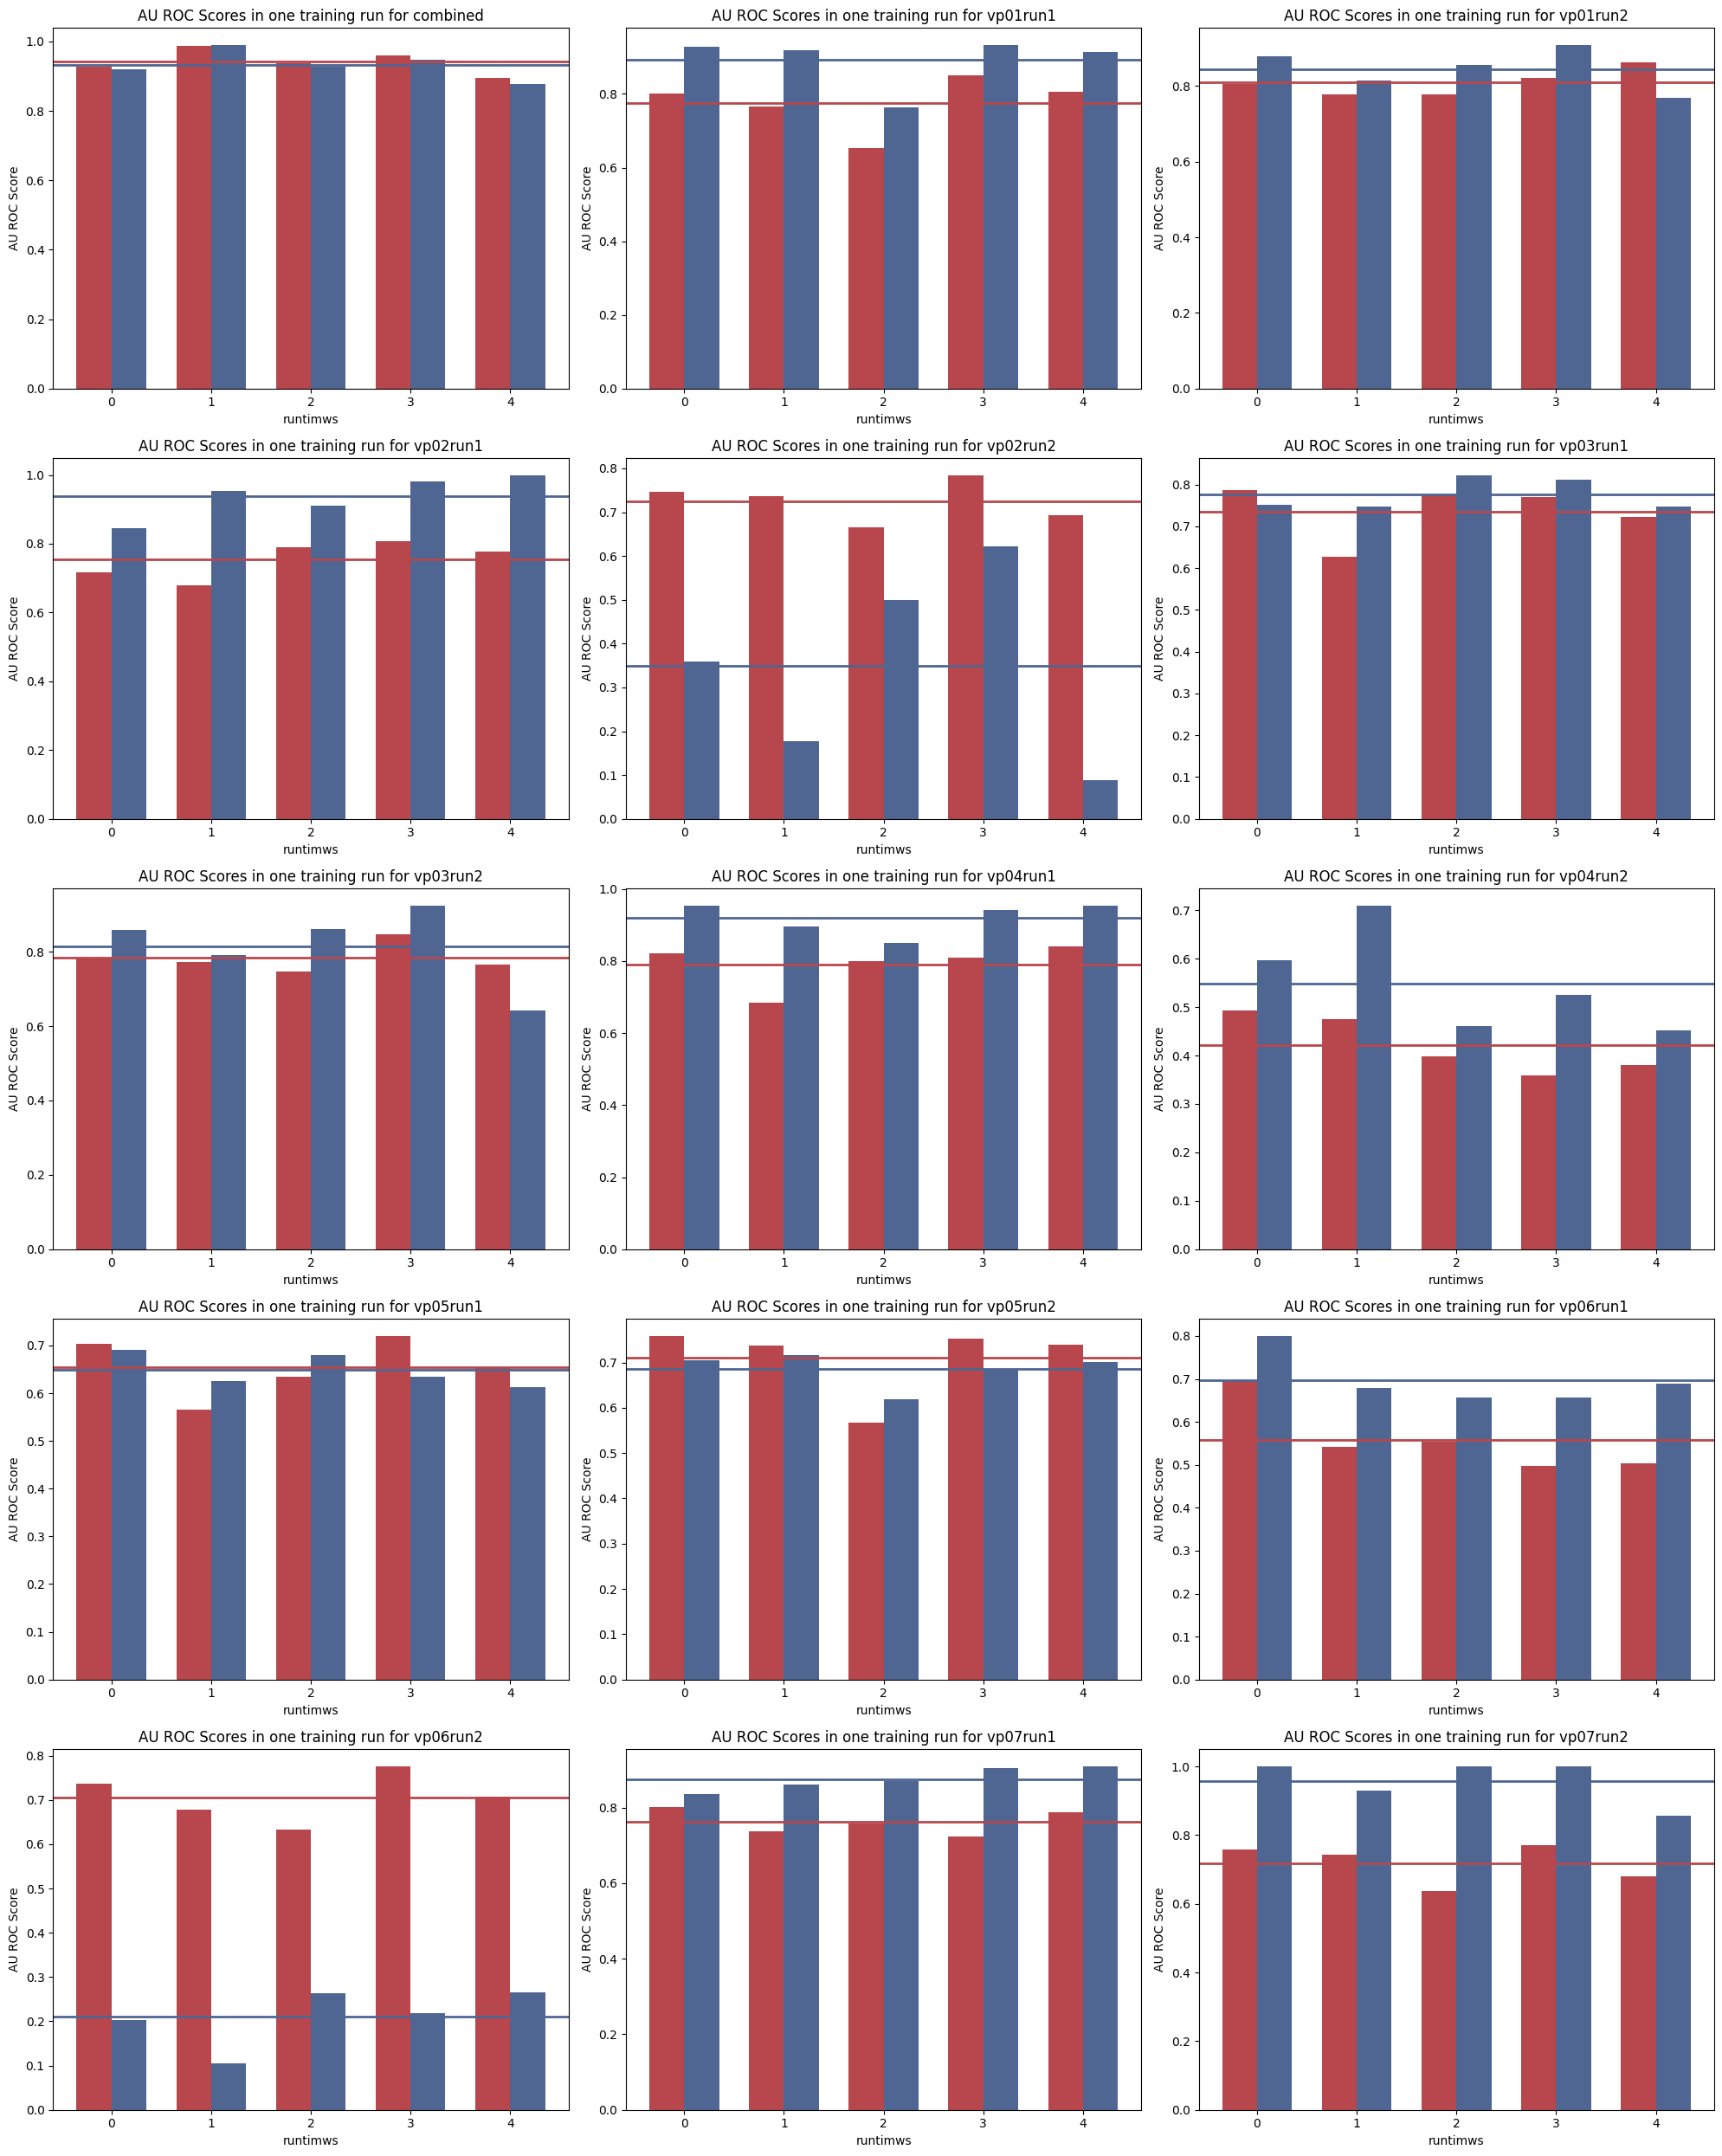
\includegraphics[width=\textwidth]{figures/05_all_results1.png}
    \caption{all the results of the model JODIE with state embedding-1} 
    \label{fig:all_results1}
\end{figure}

\begin{figure}
    \centering
    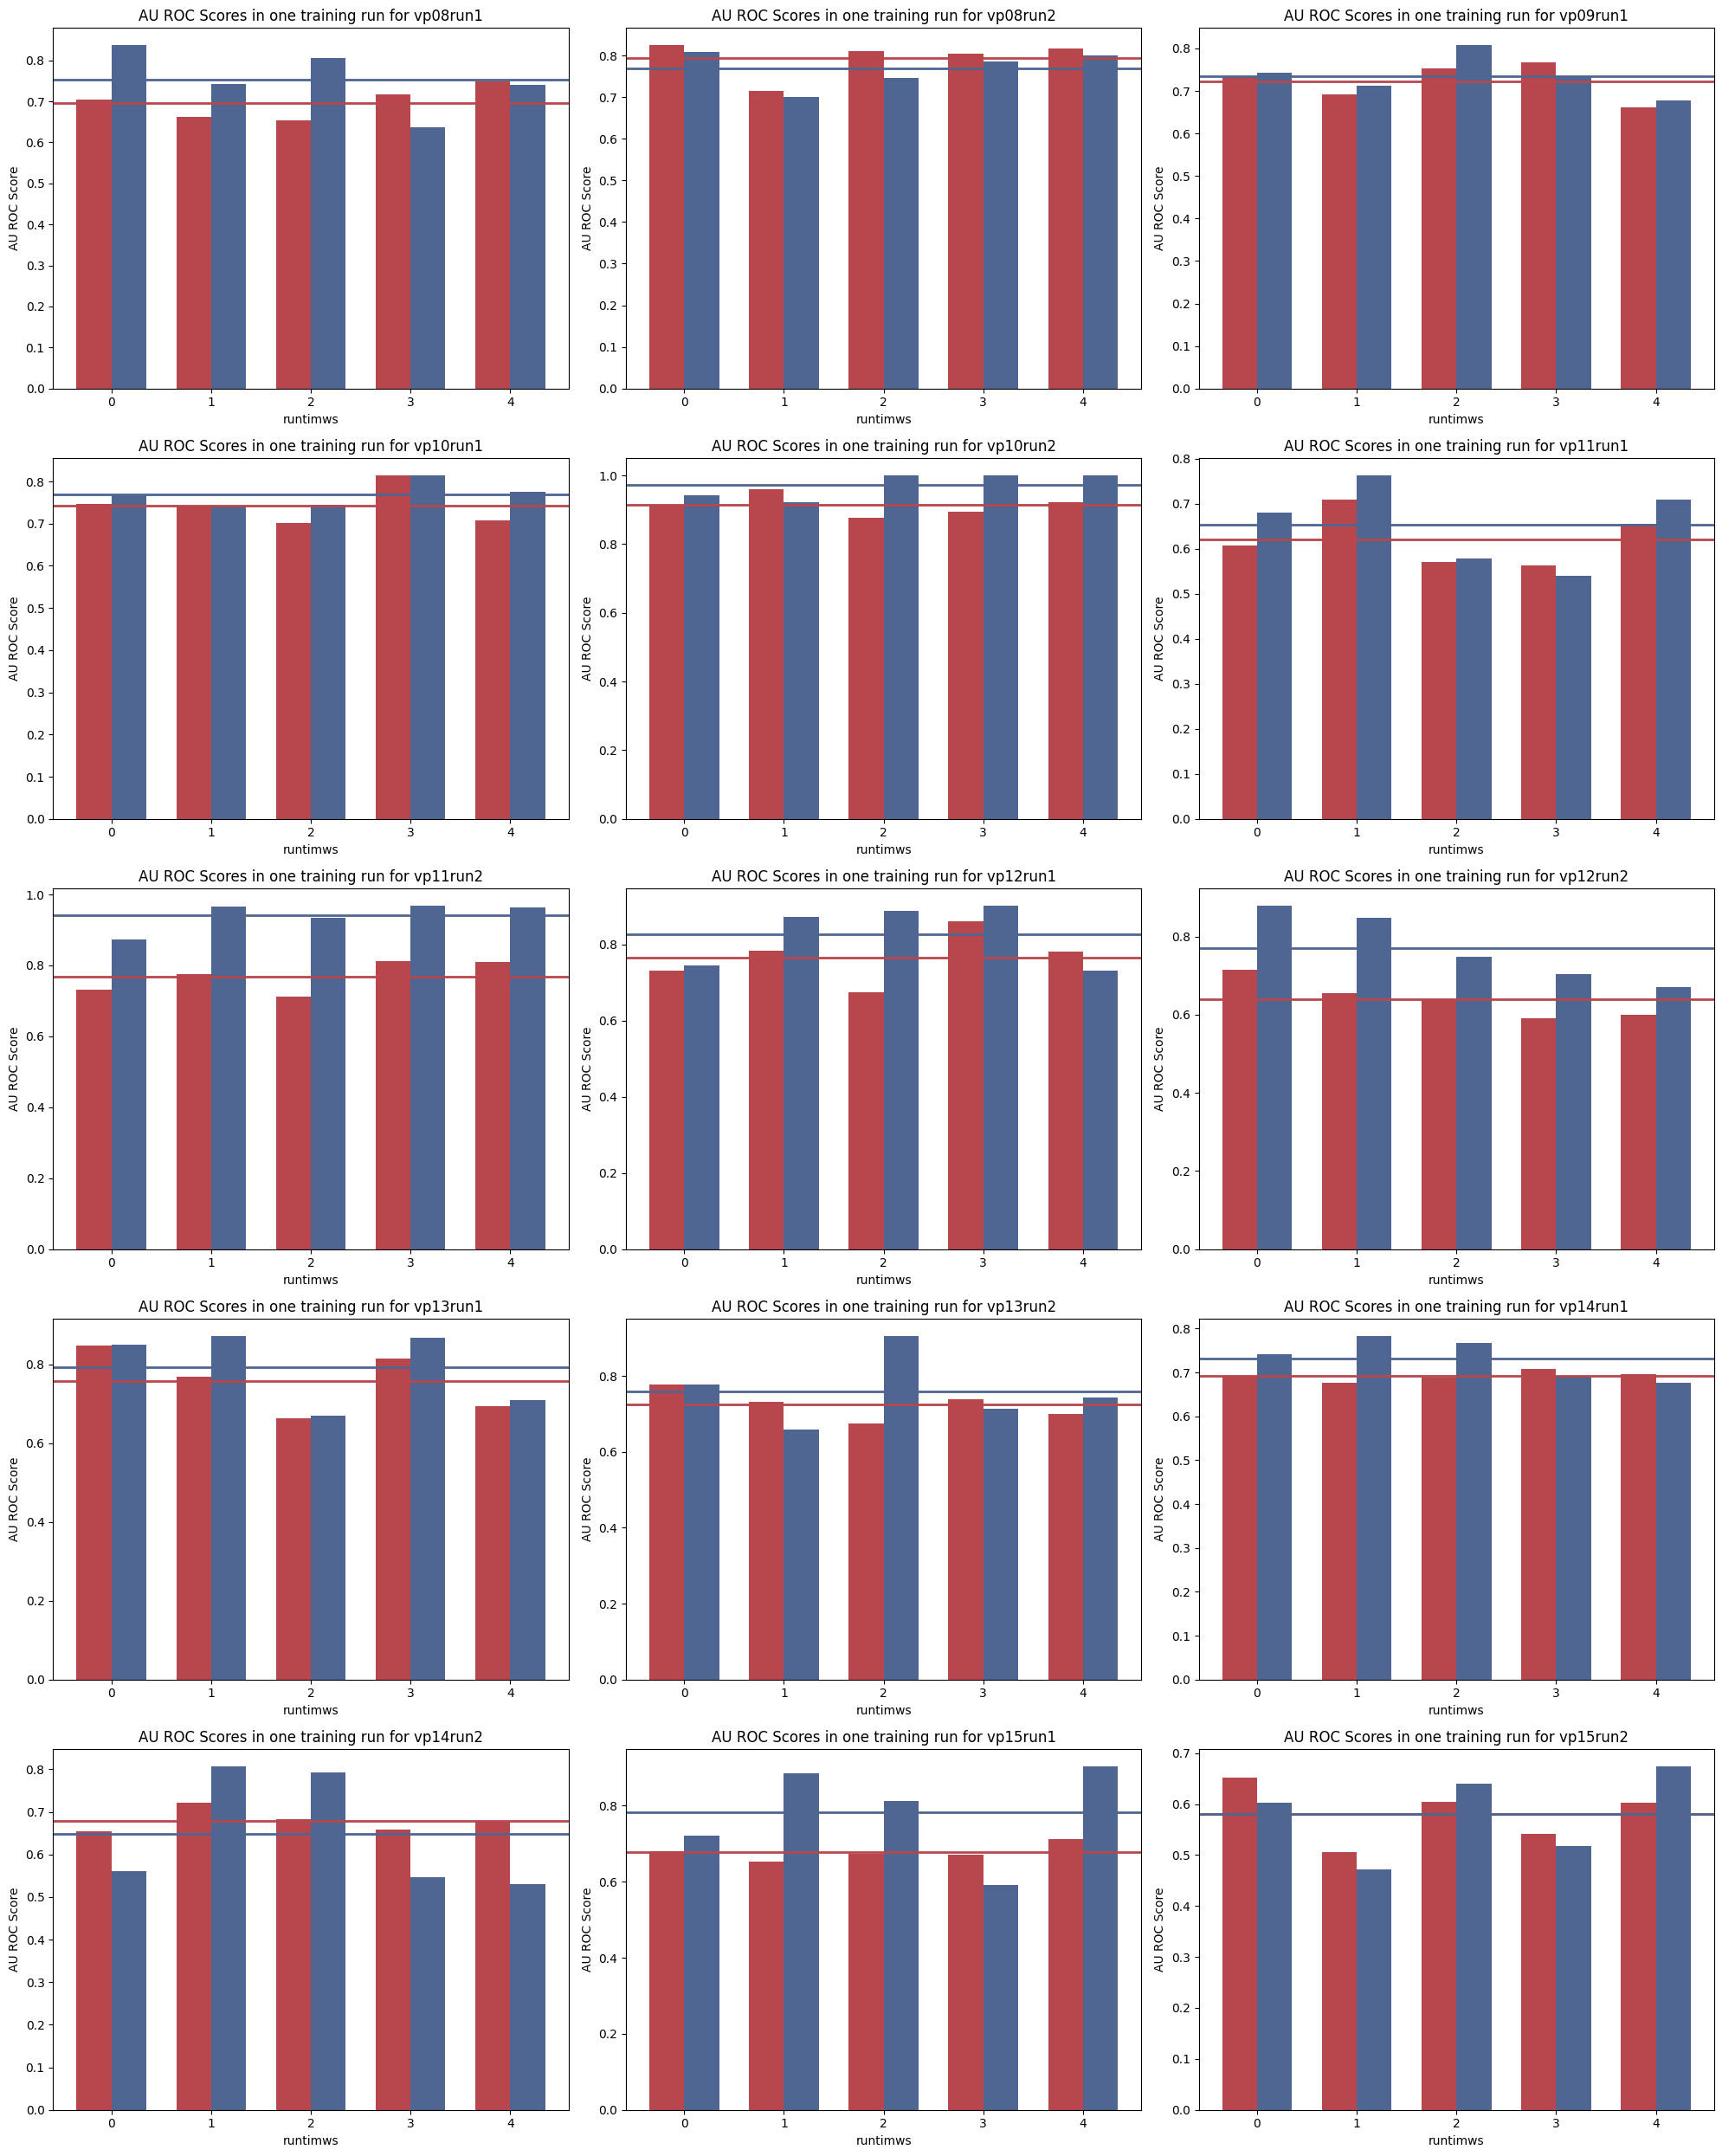
\includegraphics[width=\textwidth]{figures/05_all_results2.png}
    \caption{all the results of the model JODIE with state embedding-2} 
    \label{fig:all_results2}
\end{figure}
